\chapter{EEG/MEG preprocessing -- Reference \label{Chap:eeg:preprocessing}}

In this chapter we will describe the function and syntax of all SPM/MEEG preprocessing and display functions. This will be the most detailed description of the functions in this manual. Our goal is to provide a comprehensive description of how the software can be used to preprocess M/EEG data up to the point where one would use one of the source reconstruction techniques or statistical analysis of M/EEG channel data.

These functions can be called either from SPM's graphical user interface (GUI), from the \matlab\ command line, or via the batch input system. We recommend beginners use the GUI first, because this will prompt SPM to ask for all relevant information needed to process the data. The batch input system is designed for repetitive analyses of data (eg. from multiple subjects) once the user knows what should be done, and in which order. The command line facilities are very useful for writing scripts, or using SPM's history-to-script functionality to generate scripts automatically. The command line use of SPM for M/EEG will require some \matlab\ knowledge.

For the command line, we follow the concept of providing only one input argument to each function. This input argument is usually a structure (struct) that contains all input arguments as fields. This approach has the advantage that the input does not need to follow a specific input argument order. If an obligatory input argument is missing, the function will invoke the GUI and ask the user for the missing argument. When using the GUI, a function is called without any input argument, i.e. SPM will ask for all input arguments. If using the command line (e.g., with a script), you can specify all arguments in advance and effectively use SPM/MEEG functions in batch mode. We provide some sample batch scripts (\texttt{history\_subject1.m}) in the \texttt{man$\backslash$example\_scripts} folder of the SPM8-distribution.
\\
\\
In the following we will go through the conversion of the data, specifics of the M/EEG format in SPM8, how to properly enter additional information about the channels, how to call FieldTrip-functions from SPM, a complete reference of all methods and functions, how to use the display, and finally how to script and batch the preprocessing.

\section{Conversion of data}
The first step of any analysis is the conversion of data from its native machine-dependent format to a \matlab\-based, common SPM format. This format stores the data in a \texttt{*.dat} file and all other information in a \texttt{*.mat} file. The \texttt{*.mat} file contains the data structure \texttt{D} and the \texttt{*.dat} is the M/EEG data. The conversion facility of SPM is based on the ``fileio'' toolbox\footnote{fileio: \url{http://fieldtrip.fcdonders.nl/development/fileio}}, which is shared between SPM8, FieldTrip and EEGLAB toolboxes and jointly developed by the users of these toolboxes. At the moment most common EEG and MEG data formats are supported. For some cases, it might be necessary to install additional \matlab\ toolboxes. In this case an error message will be displayed with a link where the appropriate toolbox can be downloaded. If your data format is not recognized by ``fileio'', it will still try to read the file using the Biosig toolbox\footnote{Biosig: \url{http://biosig.sourceforge.net/}}, if available. This can work for some EEG systems, particularly clinical ones. One of the consequences of using Biosig as 'fallback' is that you may see error messages from Biosig or mentioning Biosig if your data format is not presently supported. In such a case you can extend the ``fileio'' toolbox and contribute your code to us. See ``fileio'' page for details.

In the following we will describe the GUI-version for conversion. One could also convert data using the batch or a script. After clicking on the \textsc{Convert} button of the M/EEG GUI you will be asked to select the file to be converted. As a rule of thumb, if the dataset consists of several files, the file containing the data (which is usually the largest) should be selected. SPM can usually automatically recognize the data format and apply the appropriate conversion routine. However, in some cases there is not enough information in the data file for SPM to recognize the format. This will typically be the case for files with non-specific extensions (\texttt{*.dat}, \texttt{*.bin}, \texttt{*.eeg}, etc). In these cases the header-, and not the data-, file should be chosen for conversion and if it is recognized, SPM will locate the data file automatically. Note that SPM8 can also convert data in SPM5 format, where the the \texttt{*.mat} file should be selected. In some rare cases automatic recognition is not possible or there are several possible low-level readers available for the same format. For these cases there is an option to force SPM to use a particular low-level reader available with the batch tool or in a script (see below).

After the file is chosen, you will be asked (``Define settings?'') to choose whether to define some settings for the conversion or ``just read''. The latter option was introduced to enable a simple and convenient conversion of the data with no questions asked. The resulting SPM M/EEG data file can then be explored with SPM's reviewing tool to determine the appropriate conversion parameters for the future. If the ``just read'' option is chosen, SPM will try to convert the whole dataset preserving as much data as possible. The other option - ``yes'' - lets you control all features of the conversion, to convert only the data that will be used in subsequent processing.

If this option is chosen, the next question will be whether to read the data as ``continuous'' or as ``trials''. Note that some datasets do not contain continuous data to begin with. These datasets should usually be converted with the ``trials'' option.

If the ``continuous'' option is chosen you will be asked (``Read everything?'') whether to convert the whole file (``yes'') or a subset of it (``no''). If the answer is ``no'' you will be asked to specify the time window in seconds. Note that if a data file contains several concatenated long segments (e.g., if the recording was paused and then resumed) only one of these segments at a time can be converted as continuous. Therefore you should specify a time window which does not cross the boundaries between segments.

If the ``trial'' option is selected, the next question will be where to retrieve the information about trials. There are three options. If ``data'' is chosen, SPM will attempt to look for information about trials in the dataset. This option is suitable for datasets that are already epoched or datasets which contain information about trials. If ``define'' is selected, trials can be defined based on information about events which appears in the file. The routine used for this option is identical to the one used in epoching (see below) and the resulting SPM file will be already epoched. The advantage of defining trials at conversion is that only the necessary subset of the raw data is converted. This is useful when the trials of interest are only a small subset of the whole recording. After the trial definition is completed, the results can be saved into a file. This file can be later used instead of repeating the trial definition again. This is done by selecting the third trial definition option - ``file''.

The next question will be about which channels should be converted. Five options are available. ``all'' - convert all the available channels. ``meg'', ``eeg'' - automatically detect and choose MEG and EEG channels respectively. These options may not work correctly for some EEG systems because many data formats do not provide information about what data were acquired by a specific channel. However, the most common cases are supported. ``gui'' - choose the channels to convert using a graphical interface. The overall selection of channels can be saved in a file and this file can later be used by choosing the ``file'' option.

The final question is by which name the new SPM EEG files should be written to disk. By default SPM will add the prefix \texttt{spm8\_} to the name of the raw data file if the data is read as continuous and \texttt{espm8\_} if the data is read by trials.

SPM will now convert the data. This may take some time depending on file size and a red bar will inform you about the progress.


\section{Converting arbitrary data}
It might be the case that your data is not in any standard format but is only available as an ASCII or Excel file or as a variable in the \matlab\ workspace. Then you have two options depending on whether you would be willing to use a \matlab\ script or want to only use the GUI. If you want to only use the GUI, we suggest that you assemble your dataset in EEGLAB and then  save it and convert to SPM as any other format. The developers of EEGLAB have invested a lot of effort into making it possible to build a dataset from scratch without using the command line or scripts and we see no reason for reproducing the same functionality in SPM.

If you are willing to write a simple \matlab\ script, the most straightforward way to convert your data would be to create a quite simple FieldTrip raw data structure (\matlab\ \texttt{struct}) and then use SPM's \texttt{spm\_eeg\_ft2spm.m} function to convert this structure to SPM dataset. Missing information can then be supplemented using \texttt{meeg} methods and SPM functions.

FieldTrip raw struct must contain the following fields:

\begin{itemize}
\item \texttt{.fsample} - sampling rate (Hz)
\item \texttt{.trial} - cell array of trials containing matrices with identical dimensions (channels $\times$ time). 
\item \texttt{.time} - cell array of time vectors (in sec) - one cell per trial, containing a time vector the same length as the second dimension of the data. For SPM, the time vectors must be identical.
\item \texttt{.label} - cell array of strings, list of channel labels. Same length as the first dimension of the data.
\end{itemize}

If your data only has one trial (e.g. it is already an average or it is raw continuous data) you should only have one cell in \texttt{.trial} and \texttt{.time} fields of the raw struct.

An example script for converting LFP data can be found under \texttt{toolbox$\backslash$Neural\_Models$\backslash$spm\_lfp\_txt2mat.m}.

\section{The M/EEG SPM format}
The M/EEG format has changed from SPM5 to SPM8. There were many reasons why we decided that it was time to radically change the format. If you still have some data from your SPM5 analyses, you can convert them to SPM8 (see above).

Here are the reasons why we changed the format. Previously, we placed all header information into a struct, which was then stored in a \matlab\ \texttt{mat}-file. When the data were read, the struct-file was put into working memory, and the data, contained in the \texttt{dat}-file, was linked to the struct, using memory-mapping. We found that making a struct available in working memory was highly problematic. This was because users would manipulate the struct but sometimes introduced an error to the format (e.g., they removed a few trials from the data but did not update all fields relating to the total number of trials). This would generate hard-to-resolve errors when trying to further process the now inconsistent data. To avoid this in the future, we have introduced two changes. The first is that SPM8 now always does a consistency check when loading a file. This means, if, for whatever reason, the data format was made inconsistent, SPM8 will now report this as soon the user tries to load these data. SPM8 will also report where the check flagged an inconsistency. If there is enough information available to fix the inconsistency, it will be fixed on the fly. For instance, you will usually see some messages about missing information starting with 'checkmeeg:' when converting a file to SPM8 format. These messages are normal and if no error is generated they do not indicate a problem. Second, when reading the data, we now convert the header struct to an object and only then make it available in working memory. Generally, this \matlab\ object can only be manipulated using standardized functions (called methods), which makes it very hard to introduce any inconsistency into SPM M/EEG data in the first place. Also, using methods simplifies internal book-keeping, which makes it much easier to program functions operating on the M/EEG object. For example, while the SPM5 format kept a variable which contained the number of trials, the SPM8 object does not have this variable but a method that returns the number of trials by simply counting how many trials of data there are. This makes it easy for a programmer to, for example, remove trials. There is no longer a need to update a variable for the number of trials. Also there is no need to check for the presence of particular fields in the struct in every SPM function. All the methods are guaranteed to work on a valid object. There are many more simplifications along these lines due to the use of ``objects'' and ``methods''. In summary, the change in format has resulted in a much more robust, and usable data format.

\section{Preparing the data after conversion}
SPM tries to do its best to extract information automatically from the various data formats. In some cases it can also supplement the converted dataset with information not directly present in the raw data. For instance, SPM can recognize common EEG setups (extended 1020, Biosemi, EGI) based on channel labels and assigns 'EEG' channel type and default electrode locations for these cases. However, there are data types which are either not yet supported in this way or do not contain sufficient information for SPM to make the automatic choices. Also the channel labels do not always correctly describe the actual electrode locations in an experiment. In these cases, further information needs to be supplied by the user. Reading and linking this additional information with the data is the purpose of the \texttt{Prepare} interface. This interface is accessed by selecting \texttt{Prepare} from the ``Other'' drop-down menu in the GUI. A menu (easily overlooked) will appear at the top of SPM's interactive window. The same functionality can also be accessed by pressing ``Prepare SPM file'' in the SPM M/EEG reviewing tool.

In this menu, an SPM M/EEG file can be loaded and saved using the ``File'' submenu. The ``Channel types'' submenu allows reviewing and changing the channel types. Use the ``Review'' option to examine the presently set channel types. During conversion, SPM  will make an informed \textit{guess} at the correct channel types but this can sometimes go wrong, especiallly for EEG data. To set a particular channel group to some channel type, select this type from the menu. A list of all channels will appear. Select the subset whose type you would like to set. \texttt{Ctrl} and \texttt{Shift} buttons can be used to refine the selection. Press OK to apply your choice. It is especially important to correctly specify which are the EEG channels. MEG types are assigned automatically by SPM and cannot be modified using the GUI.

The ``Sensors'' submenu can be used to supply information about the sensor positions to the file. This information is needed to perform 3D
source reconstruction and DCM analysis for EEG and MEG data. Sensor positions for MEG are extracted from the raw data automatically and are already present. For EEG, sensor positions are usually measured by a special device (such as Polhemus) and are not part of the dataset. Even if you do not measure electrode positions routinely in your lab, we recommend to perform at least one initial measurement with the electrode cap you use and use the result as your standard template. In order for SPM to provide a meaningful interpretation of the results of source reconstruction, it should link the coordinate system in which sensor positions are originally represented to the coordinate system of a structural MRI image (MNI coordinates). In general to link between two coordinate systems you will need a set of at least 3 points whose coordinates are known in both systems. This is a kind of \textit{Rosetta stone}  that can be used to convert a position of any point from one system to the other. These points are called ``fiducials'' and the process of providing SPM with all the necessary information to create the \textit{Rosetta stone} for your data is called ``coregistration''. The most commonly used fiducials are the nose bridge and the two pre-auricular points. The coordinates of these points for SPM's standard template image are hard-coded in SPM code. So if you provide the coordinates of these specific points with your sensor positions, it will be enough for SPM. If you do not have these fiducials but have other anatomical landmarks (for instance 3 EEG electrodes whose positions can be easily marked on a structural image) it will be possible to use them for coregistration as well, but that will require additional input from you. In addition, or as a replacement of fiducials a headshape measurement may be used. This measurement is done by an operator moving his digitizer pen around on the subject's scalp and generates many more data points than just 3 fiducials. EEG sensor and fiducial positions can be added to an SPM file using the ``Load EEG sensors'' menu. There are 3 options:

\begin{itemize}
\item	``Assign default'' - assigning default sensor positions. If this is possible, it will be done automatically at conversion but this option can be used to revert to default sensor positions after making some changes.

\item ``From a \texttt{*.mat} file'' - this option is for the kind of files that were used in SPM5 and can also be used for any kind of locations without trying to get them into one of the standard formats. SPM will ask for two files. The sensors file should contain an $N \times 3$ matrix, where $N$ is the same as the number of channels whose type is set to ``EEG'' and the order of the rows matches the order of these channels in the SPM file. The fiducials file should contain a $K \times 3$ matrix, where $K$ (usually 3) is the number of fiducials. You will then be asked to provide labels for these fiducials. They should appear in the same order as the rows in the file.

\item	``Convert locations file'' - this option uses a function from the internal ``fileio'' toolbox that supports several common formats for EEG channel position specification such as \texttt{*.sfp} and BESA's \texttt{*.elp}. It can also read Polhemus files from FIL and FCDC. In general Polhemus devices do not have a standard data format so if you are using Polhemus at a different site is is most likely that your Polhemus file will not be recognized by SPM directly. You will need to convert it to another format. An \texttt{*.sfp} file is the easiest to create (for instance in Excel). It is just an ASCII file containing a column of channel labels and 3 columns of cartesian coordinates. Check ``fileio'' website\footnote{fileio: \url{http://fieldtrip.fcdonders.nl/dataformat}} for a complete list of supported formats. The file you are importing can also contain positions of fiducial points or any other named points that do not necessarily correspond to channels. You can also include multiple headshape points with the label ``headshape''. The important thing is that there are coordinates for each channel that was assigned ``EEG'' type.

\end{itemize}

The fiducials for MEG are automatically loaded from the dataset. However, in some MEG setups the situation is more complicated. For instance, it might be convenient to attach the coils marking MEG fiducials to the top of the head, where there are no clear anatomical landmarks. In this case there should be an additional file measured with a Polhemus-like device that contains the positions of MEG fiducials and something that can be linked to a structural image (either anatomical landmarks or a headshape) in the same coordinate system. The way SPM handles this situation is in two steps. First, this additional file is converted into the same coordinate system in which MEG sensors are represented and it replaces the original MEG fiducials. At a later stage having MEG sensors and fiducials/headshape in the same coordinate system, SPM uses the fiducials/headshape for coregistration with standard MRI template or subject's own structural image. If you can mark the points where your MEG fiducial coils were located on a structural image, the step described below is not necessary. It is also possible that the digitizer measurement is stored with the raw data. Then SPM will read it automatically. Otherwise, the additional fiducials/headshape file can be loaded using the ``Load MEG Fiducials/Headshape'' menu. The supported formats are the same as for electrode locations. It is also possible to create a fiducials/headshape \matlab\ struct and store it in a \texttt{*.mat} file. This file will also be recognized by SPM. The struct should be called \texttt{shape} and it should contain the following fields: \texttt{shape.pnt} - a $K \times 3$ matrix (possibly empty) with headshape points i.e. points that are on the surface of the head and have no labels, \texttt{shape.fid.pnt} - $M \times 3$ matrix with fiducial points i.e. points that have labels, \texttt{shape.fid.label} - $M \times 1$ cell array of strings with the labels of the points in \texttt{shape.fid.pnt}. As mentioned above, $M$ should be at least 3 for the coregistration to work.

If you did not use default 3D positions, after loading the sensor positions you can perform coregistration of your sensors with SPM's template head model. This initial alignment is helpful to verify that the sensor information you supplied were interpreted correctly and should also be done if you would like to generate a 2D sensor template based on your 3D sensor positions (see below). The 2D-coordinates will be used for displaying the data in a topologically meaningful way. This is implemented using the ``Coregister'' option. For details of how this option works see the 3D source reconstruction chapter \ref{Chap:eeg:imaging}.

The ``2D Projection'' menu deals with the generation of representative 2D-coordinates for the sensors. Note that generating 2D-coordinates is
not obligatory. If the 2D-coordinates are not specified, the sensors will be, when displaying, presented in a default square grid. Missing out
on topographically meaningful 2D-coordinates might be useful when working on few channels. The 2D-coordinates are also used for producing scalp-level SPMs in voxel space when converting M/EEG data to images for later statistical analysis (see below). If you are
planning to do 3D source reconstruction or DCM, 2D-coordinates are not necessarily required. Also, you can load 2D-coordinates from a file (several example files are available in the \texttt{EEGtemplates} SPM directory). 2D-coordinates can also be generated by projecting the 3D sensor positions to a plane. This is done automatically when default 3D coordinates can be assigned, and also for MEG. In case of custom EEG sensor positions coregistration should be performed first (see above). The resulting 2D-coordinates are displayed in SPM's graphics window. You can modify these projected 2D-coordinates manually by adding, deleting and moving sensors. To select a sensor, click on its label. The label will change its color to green. If you then click at a different location, the sensor will be moved to this position. Note that, at this stage, SPM does not check whether there is any correspondence between the labels of the coordinates and the labels of the channels stored in the SPM file. When you are satisfied with the 2D-coordinates, select ``Apply'' from the menu and the coordinates will be assigned to EEG or MEG channels according to their labels. Note that 2D-coordinates cannot be assigned to channels of other types than M/EEG.

Remember to save the file using ``File/Save'' after you finished modifying it using the \texttt{Prepare} interface. Your changes will not be saved automatically. In case of invoking \texttt{Prepare} from the reviewing tool you should press the 'OK' button that will appear at the bottom left of the interactive window, and then save the file with the ``Save'' button of the reviewing tool.

In the rare case that you neither have measured sensor locations, or fiducials, and the supplied standard templates do not work for you, you can also supply a so-called channel template file, which contains all information necessary. However, remember, that if you do not supply any 2D-coordinates, you can still use all SPM functions, however, SPM will use 2D-coordinates laid out in a topographically unmeaningful rectangular pattern.

A channel template file contains four variables:\\

\begin{tabular}{llcp{9cm}}

{\bf \texttt{Nchannels}} & &  - & The number of channels\\

{\bf \texttt{Cnames}}&  & - & A cell vector of channel names. Each cell can contain either a string or a cell vector of strings. The latter allows
for multiple versions of a given channel name. Case can be ignored, i.e., it doesn't matter whether channel names are in small or capital letters.\\

{\bf \texttt{Cpos}} & & - & A $2 \times Nchannels$-matrix of channel coordinates on a 2D plane. In $x$- and $y$-direction the minimum coordinate must be $\leq 0.05$ and the maximum coordinate must be $\geq 0.95$. \\

{\bf \texttt{Rxy}} & & - & A factor that determines the ratio of the width of the display plots to their height when displaying the data. Standard is $1.5$. \\

\end{tabular}

Note that the channel template files and 3D coordinate files with labels (such as \texttt{*.sfp}) can contain many more channel labels than your data file. SPM searches, for each channel in the data, through the labels in the channel template file. If the labels match, the coordinate is used.

\section{Integration of SPM and Fieldtrip}
The SPM8 distribution includes the latest version of the FieldTrip toolbox\footnote{FieldTrip: \url{http://fieldtrip.fcdonders.nl/}}. FieldTrip is a \matlab\ toolbox for MEG and EEG analysis that is being developed at the F.C. Donders Centre (FCDC) together with collaborating institutes. FieldTrip functions can be used for many kinds of analysis which are not supported in SPM proper. However, FieldTrip does not have extensive graphical user interface and its functionality should be accessed by writing scripts. Full reference documentation for FieldTrip including example scripts is available at the FieldTrip website. The SPM distribution also contains some documentation, contained as help comments in FieldTrip functions. These can be found in the directory \texttt{external$\backslash$fieldtrip}. 

Fieldtrip data structures can be converted to SPM EEG files using the \texttt{spm\_eeg\_ft2spm} function. SPM M/EEG data, once loaded with the function \texttt{spm\_eeg\_load} can be converted to FieldTrip format using the methods \texttt{ftraw} (with syntax \texttt{D.ftraw} or \texttt{ftraw(D)}) and \texttt{fttimelock} (with syntax \texttt{D.fttimelock} or \texttt{fttimelock(D)}). For SPM time-frequency datasets \texttt{fttimelock} method converts the data to Fieldtrip time-frequency structure.

\section{Reading of data\label{sec:load}}
If you use the GUI only, there is no need to read this section because the functions called by the GUI will read the data automatically. However, if you plan to write scripts and access the data and header information more directly, this section should contain all the necessary information to do so.

An SPM8 for M/EEG file can be read using the \texttt{spm\_eeg\_load} function. Without any arguments a file requester asks for the name of the file. With a string argument $P$, \texttt{spm\_eeg\_load(P)} will attempt to read a file with the name \texttt{P}. The behavior in this case is identical to the ``Just read'' option in the GUI. The SPM-format stores the binary data in a \texttt{*.dat} file. All header information are stored in a \texttt{*.mat} file. This \texttt{*.mat} file contains a single struct named \texttt{D} which contains several fields. When using \texttt{spm\_eeg\_load}, the struct is transformed into an object, and the data are linked into this object. The linking is done via memory mapping using \texttt{file\_array} objects. Note that the data should always be read using the routine \texttt{spm\_eeg\_load}. The memory mapped data can be addressed like a matrix (see below) which is convenient for accessing the data in a random access way. However, a word of caution: If you write new values to this matrix, the matrix is not only changed in the object (in memory), but also physically on the hard disk.

You can also load the header struct using a simple \matlab\ \texttt{load} but this just returns the header struct, without the data linked in, and SPM functions won't know what to do with this struct. In the following, we will describe the methods that one can use on an M/EEG-object. Note that we will not describe the internal format of the data here. This would be helpful only for programmers who want to write new methods for \texttt{meeg} object, because when simply analyzing M/EEG or even writing SPM functions there should never be a need to access the internal format. If you think that the existing methods do not provide the functionality you need, please let us know. For interested power users, there is documentation about the internal format within the \texttt{meeg} class constructor.
\textit{meeg}.

\subsection{Syntax}
\texttt{D = spm\_eeg\_load(P)}
\\

\subsubsection{Input}
The input string \texttt{P} is optional and contains the file name of the \texttt{*.mat} file.

\subsubsection{Output}
The output struct \texttt{D} contains all header information about the data. The data are memory mapped and can be accessed directly using something like \texttt{d = D(:,:,1)}. This command would put the first trial over all channels and time points into the variable \texttt{d}. The first dimension of \texttt{D} is channels, the second peri-stimulus time, and the third is trials. If the data are time-frequency transformed, there would be four dimensions, where the frequency dimension is squeezed in at the second position (i.e., channels/frequencies/time/trials). If you wanted to change the values of the data, you would write something like \texttt{D(1,2,3) = 1;}, which would change the value of the first channel, second time-point, and third trial to 1.


\section{Methods for the \texttt{meeg} object}
\texttt{meeg} methods are functions that operate on an \texttt{meeg} object, loaded with \texttt{spm\_eeg\_load}. These methods should not be used, if you just want to analyze your data using the GUI or simple scripts. However, if you write your own scripts or high-level functions that need to read or manipulate the object, you need these methods. In the following, we will provide details about most of the methods. The code for all methods can be found in the \texttt{@meeg} SPM directory. Most methods provide some minimalist help text. In the following, we will assume that the object variable is called \texttt{D}, i.e. previously loaded by using \texttt{D = spm\_eeg\_load;}.

\subsection{Constructor \texttt{meeg}}
The \texttt{meeg} method is a constructor. Called without any arguments it will produce a consistent, but empty object. In SPM, the constructor is called when a struct has been loaded into memory by \textit{spm\_eeg\_load}, and is transformed into an \texttt{meeg} object. Importantly, the constructor also checks the consistency of the object.

\subsection{display}
This method will return, in the \matlab\ window, some information about the object, e.g., \texttt{display(D)}.

\subsection{Number methods}
These are methods which return the number of something; they count the number of channels, etc. For example, to find out how many channels an MEEG object contains, you would use \texttt{D.nchannels}, where $D$ is the object. Number functions are \texttt{nchannels, nfrequencies, nsamples, ntrials}. You can also use \texttt{size(D)} to get all the dimensions of the data array at once.

\subsection{Reading and manipulation of information}
There are a large number of methods that can be used to either read or write some information. The method name is the same but it depends on the arguments whether something is read or stored. For example, when you use the method \texttt{badchannels}, you can either type \texttt{D.badchannels}, which returns the indices of all bad channels. You could also change information about specific bad channels, e.g., \texttt{D.badchannels([43:55], 1)} will flag channels 43 to 55 as bad. You   could also use \texttt{D.badchannels([43:55], ones(1,13)}, i.e. you can either use a scalar to change all channels listed, or supply a 0/1-flag for each channel. There are other functions which use the same logic. In the following we will list these functions and describe briefly what they do but won't go into much detail. We believe that you can work it out using the badchannels-example.

\subsubsection{selectdata}
With this method the data can be indexed using channel labels, times and condition labels instead of indices which you would usually need to find out in your code. For instance \texttt{D.selectdata('Cz', [0.1 0.12], 'Oddball')} will return the waveforms of channel Cz between 100 and 120 ms in peristimulus time for the condition ``Oddball''.

\subsubsection{chanlabels}
This method reads or writes the label of the channels (string).  Note that the channel labels must be unique.

\subsubsection{chantype}
This method reads or writes the type of a channel (string). Currently, the types recognized by SPM are: ``EEG'', ``MEG'', ``EMG'', ``EOG'', or ``Other'', but in principle type can be any string.

\subsubsection{conditions}
This method  reads or writes the name of the condition of an epoch (string).

\subsubsection{events}
This method returns the events stored with each trial. Events are records of things that happened during the experiment - stimuli, responses, etc. Before a file is epoched all the events are stored with the only trial and they can be used by the epoching function. For an epoched file SPM stores with each trial the events that occured within that trial or possibly in some time window around it (this is a parameter of the epoching function that can be specified). You can use this information for your analysis (for instance to sort trials by reaction time). Events are represented by a structure array with the following fields:

\begin{itemize}
\item \texttt{.type} - string (e.g. ``front panel trigger'')
\item \texttt{.value} - number or string, can be empty (e.g. ``Trig 1'').
\item \texttt{.time} - in seconds in terms of the original file
\item \texttt{.duration} - in seconds (optional)
\end{itemize}

Note that in order to find out the time of an event in peristimulus time you will need additional information provided by ``trialonset'' method.

\subsubsection{fname}
This method reads or writes the name of the \texttt{mat}-file, in which the header information are stored.

\subsubsection{fnamedat}
This method reads or writes the name of the \texttt{dat}-file, in which the data are stored.

\subsubsection{frequencies}
If the data has been transformed to time-frequency, this method reads or writes the frequencies (Hz) of the data.

\subsubsection{fsample}
This method reads or writes the sampling rate of the data. In SPM, all data must have the same sampling frequency.

\subsubsection{history}
This method can read or add to the history of a file. Usually, each time a SPM function (e.g. like converting) does something to a data set, the function name and arguments (possibly after collecting them with the GUI) are stored in the history. Effectively, the history is a documentation of how exactly the data were processed. Of course, the history function can also be used to replicate the processing, or generate (modifiable) scripts for processing other data in the same way.

\subsubsection{path}
This method reads or writes the path, under which the \texttt{mat}- and \texttt{dat}-files are stored.

\subsubsection{reject}
This method reads or writes the indices of rejected (bad) trials.

\subsubsection{timeonset}
This method reads and writes the time of the first sample in a trial in peristimulus time (in seconds). In SPM all trials should have the same time axis. Therefore there is only one timeonset in a file. For instance, if you have a pre-stimulus baseline of 100 ms and the stimulus comes at time zero, \texttt{timeonset} will be -0.1. In general it is possible to define the time axis any way you like and there is no requirement that the stimulus comes at 0 or that there is baseline with negative times (which was the case in SPM5).

\subsubsection{trialonset}
This method should not be confused with the more commonly used \texttt{timeonset} (see above). It returns the times of the first sample of each trial in the original raw data file time. This information is not always available to begin with. It may also be invalidated during processing (for instance if you merge two epoched files). When this happens the information is discarded. For SPM analysis \texttt{trialonset} is not usually necessary. However it may be useful if you want to relate something in your analysis to the timing of your experiment, for instance create a regressor for GLM analysis of single trials to account for fatigue. \texttt{trialonset} is also necessary for interpretation of events in epoched files.

\subsubsection{transformtype}
This method reads and writes the type of the data transform (string). For example, when the data are transformed to a time-frequency represention, \texttt{transformtype} is set to ``TF''. For time data, this is ``time''.

\subsubsection{type}
This method reads and writes the type of the data (string). Currently, this string can be ``continuous'', ``single'', ``evoked'', or ``grandmean''.

\subsubsection{units}
This method reads and writes the units of the measurements (string). The units are channel-specific, i.e., each channel can have its own units.

\subsection{Reading of information}
Some methods can only read information but not change them. These are:

\subsubsection{condlist}
This method returns a list of condition labels. Multiple entries of labels have been removed.

\subsubsection{coor2D}
This method returns the 2D-coordinates used for displaying or writing sensor data to voxel-based images.

\subsubsection{dtype}
This method returns the type under which the data are stored in the \texttt{file\_array} object.

\subsubsection{eogchannels}
This method returns which of the channels are EOG channels.

\subsubsection{indsample}
This method returns the index of the sample which is closest to a specific time point (ms).

\subsubsection{indfrequency}
For time-frequency datasets this method returns the index of the frequency closest to the given value in Hz.

\subsubsection{indchannel}
This method returns indices of channels based on their labels.

\subsubsection{indtrial}
This method returns indices of trials based on condition labels.

\subsubsection{meegchannels}
This method returns the indices of all channels that are either of the MEG or EEG type.

\subsubsection{modality}
This method returns the modality of channels (MEG, EEG, etc.).

\subsubsection{pickconditions}
This method returns the indices of trials of a certain condition. The condition must be supplied by its label (string).

\subsubsection{repl}
This method returns the number of replications measured for a condition. This method is usually only used on single trial data.

\subsubsection{time}
This method returns the time (ms) of the samples.

\subsubsection{sensors}
This method returns the sensor locations structure. There is an additional argument for modality ('EEG' or 'MEG') as we are planning to support datasets with more than one sensor type. The exact way sensors are represented depends on the modality and you can find more information in Fieldtrip documentation as the sensors structure is produced and used by code originally developed at FCDC. Note that in SPM, sensors are not directly linked with channels, unlike for instance in EEGLAB. So there is no requirement for the number of sensors and channels to match or even for any relation between them. Of course loading sensors completely unrelated to your data will not be very useful and will eventually lead to an error. This kind of representation is more powerful than a simple correspondence and it will become even more useful with further development of SPM.

\subsubsection{fiducials}
This method returns the fiducials. They are represented as \texttt{shape} struct (see the discussion of loading fiducials by the \texttt{Prepare} function) with an additional field for units that is assigned automatically.

\subsubsection{ftraw}
This method converts an object to a FieldTrip structure. An additional argument can be supplied to indicate whether the data is memory mapped (1: default) or loaded into memory (0). Note that not all FieldTrip functions can properly handle memory mapped data. In order to avoid corrupting the data, \texttt{ftraw} sets a read-only flag on it so in the worst case you might encounter errors in Fieldtrip functions. Please report such errors on the SPM or Fieldtrip mailing list so that we can fix them. \texttt{ftraw(0)} is safer in this respect but inefficient in its memory use.

\subsubsection{fttimelock}
Similar to \texttt{ftraw} but converts the data to a different kind of Fieldtrip structure. 

\subsection{Changing the information saved on the disk}

\subsubsection{save}
This method saves the object to the \texttt{mat}- and \texttt{dat}-files.

\subsubsection{delete}
This function deletes the \texttt{mat}- and \texttt{dat}-files from the disk. This is useful, for instance, in a script to delete the intermediate datasets after the next processing step has been completed. 

\subsection{struct-like interface}
In addition to pre-defined internal fields that should only be manipulated using methods, the \texttt{meeg} object also allows storing additional information in it as long as the names of additional fields do not clash with the names of existing methods. This functionality is used by some SPM functions. For instance, the results of 3D source reconstructions are stored in \texttt{D.inv} field for which no methods are necessary to access and modify it. You can use this functionality in your scripts (try commands like \texttt{D.myfield = 'hellow world'; disp(D.myfield);}). The methods \texttt{rmfield} and \texttt{isfield} work for these extra-fields as they would if the \texttt{meeg} object was a struct.

\section{SPM functions}
In this section we will describe the high-level SPM functions which are used for preprocessing M/EEG data. These functions are fairly standard and should allow a simple preprocessing of the data (e.g., epoching, filtering, averaging, etc.). Here, we will just describe what each function roughly does and what the input arguments mean. More detailed information about the syntax can be found in the help text of the code. For example, to get detailed help on epoching, type \texttt{help spm\_eeg\_epochs}. The general syntax is the same for all functions. If called from the command-line, and if no input arguments are specified, the function will behave exactly as if you called the function from the GUI by pressing a button or choosing it from the ``Other'' menu. However, on the command line, or from a script, you can supply input arguments, up to the point when all required input arguments are specified, so that the function will run without any user interaction. In this way, one can write a script that runs without user interaction. See the folder \texttt{man$\backslash$example\_scripts} for an example. Input arguments are provided in a struct \texttt{S}, whose fields contain the arguments. A typical call, e.g., from a script would be: \texttt{D = spm\_eeg\_epochs(S)}, where $S$ is the input struct, and \texttt{D} contains the return argument, the epoched \texttt{meeg} object. Note that, with all SPM functions, the object is also always written to hard disk. The filenames of the \texttt{mat}- and \texttt{dat}-files are generated by prepending a single letter to the old file name. In the example of epoching this would be an \textit{'e'}. The idea is that by calling a sequence of functions on a file, the list of first letters of the file name shows (roughly) which preprocessing steps were called to produce this file. Note that another way of calling SPM functions and specifying all input parameters is to use the new batch interface.

\subsection{Epoching the data: \texttt{spm\_eeg\_epochs}}
Epoching cuts out little chunks of continuous data and saves them as ``single trials''. In M/EEG research, this is a standard data selection procedure to remove long gaps between each single trial. For each stimulus onset, the epoched trial starts at some user-specified pre-stimulus time and end at some post-stimulus time, e.g. from -100 to 400 milliseconds in peri-stimulus time. The epoched data will also be baseline-corrected, i.e. the mean of the pre-stimulus time is subtracted from the whole trial. The resulting event codes are the same as saved in the \texttt{*.mat} file. The prepended output letter is \textit{'e'}.

The epoching function can deal with two different ways of specifying trials you want to epoch. The first is to specify explicitly where each trial is located in the measured time-series. The second is to specify trials using the labeled events stored in the file. For most users, the second way is the most convenient, but sometimes, when the stored triggers in the file do not relate to what you want to epoch or there is no event information available in the raw data (e.g. when you have an external stimuli file), you should use the first.

For the first method, you specify a $N \times 2$ so-called \texttt{trl} matrix, where each row contains the start and end of a trial (in samples). Optionally, there can be a third column containing the offset of the trigger with respect to the trial. An offset of 0 (default) means that the first sample of the trial corresponds to the trigger. A positive offset indicates that the first sample is later than the trigger, a negative offset indicates that the trial begins before the trigger. In SPM the offset should be the same for all trials. The need to specify a whole column is for interoperability with FieldTrip where trials can have different time axes. In addition you have to specify \texttt{conditionlabels} (a single string or a cell array of strings), either one for each trial or one for all trials. You can also enter a \texttt{padding} which will add time points before and after each trial to allow the user to later cut out this padding again. This is useful, e.g., for filtering epoched data, where one would otherwise, without padding experience ``edge effects''.

For the second method, one should define the pre- and post-stimulus interval, and also specify the events (triggers) around which the epochs will be ``cut''. SPM identifies events by their ``event type'' and ``event value''. These are strings or numbers which the software run by the EEG or MEG vendor uses when generating the measurement file. If you don't specify parameters for the epoching function, a GUI will pop up, and present the found triggers with their type and value entries. These can sometimes look strange, but if you want to run a batch or script to do the epoching, you have to first find out what the type and value of your event of interest are. Fortunately, these tend to be the same over scanning sessions, so that you can batch multi-subject epoching using the types and values found in one subject. You also have to come up with a ``condition label'' for each trial type, which can be anything you choose. This is the label that SPM will use to indicate the trial type of a trial at later processing stages. It is possible to use several types of triggers for defining trials with the same label - in the GUI, just select several events using \texttt{Shift} or \texttt{Ctrl} key.

For both methods of input you also have to set a (0/1)-flag (no/yes) indicating whether you want to review the information for all trials after selecting them. This allows you to make sure that all your trials are there. You should set the review-flag to 0, if you write a non-interactive script. In the GUI you can review a list of the epochs you defined and exclude some of them by hand (e.g. only take the triggers from the first 5 min of recording). You can also choose to save the trial definitions, for example, for re-use of another epoching of the same data.

\subsection{Filtering the data: \texttt{spm\_eeg\_filter}} 
Continuous or epoched data can be filtered, over time, with a low-, high-, stop- or bandpass-filter. SPM uses a Butterworth filter to do this. Note that SPM uses the signal processing toolbox. This means that you have to have this toolbox to filter data in SPM. Phase delays are minimised by using \matlab\ 's \texttt{filtfilt} function which filters the data twice, forwards and backwards. The prepended output letter is \textit{'f'}.

When you use the function in GUI mode, it will automatically
use the Butterworth-filter. You can then choose among the four different types of filtering: ``lowpass'', ``highpass'', ``bandpass'',
and ``stopband''. Depending on your choice, SPM will ask for the cutoff(s) in Hz.

\subsection{Baseline correction: \texttt{spm\_eeg\_bc}} 
This function subtracts the baseline from channel data. You will be asked to specify the baseline period in ms (e.g. [-100 0]). A new dataset will be written out with the name prepended by \textit{'b'}.

\subsection{Artefact detection and rejection: \texttt{spm\_eeg\_artefact}}
Some trials not only contain neuronal signals of interest, but also a large amount of signal from other sources like eye movements or muscular activity. These signal components are referred to as artefacts. There are many kinds of artefacts and many methods for detecting them. The artefact detection function in SPM is, therefore, extendable and can automatically detect and use plugin functions that implement particular detection algorithms. Simple algorithms presently implemented include thresholding of the data, thresholding of the difference between adjacent samples (to detect jumps), thresholding peak-to-peak amplitude and detection of flat segments. Channels containing artefacts in large proportion of the trials are automatically marked as bad. 

Note that the function only indicates which trials are artefactual or clean and subsequent processing steps (e.g. averaging) will take this information into account. However, no data is actually removed from the \texttt{*.dat} file. The \texttt{*.dat} file is actually copied over without any change. The prepended output letter is \textit{'a'}.

The GUI for artefact detection is based on the batch interface of SPM. When you click the \textsc{Artefacts} button, window of the SPM8 batch interface will open. Click on ``File name'' and select the dataset.  Double click ``How to look for artefacts'' and a new branch will appear. It is possible to define several sets of channels to scan and one of the several different methods for artefact detection. For each detection method there are specific configuration parameter (e.g. for thresholding - the threshold value).

\subsection{Downsampling: \texttt{spm\_eeg\_downsample}}
The data can be downsampled to any sampling rate. This is useful if the data was acquired at a higher sampling rate than one needs for making inferences about low-frequency components. For example, resampling from 1000 Hz to 200 Hz would cut down the resulting file size to 20\% of the original file size. Note that SPM's downsampling routine uses the \matlab\ function \texttt{resample}, which is part of the signal processing toolbox. The prepended output letter is \textit{'d'}.

Here, you choose the new sampling rate (Hz) which must be smaller than the old sampling rate.

\subsection{Rereferencing: \texttt{spm\_eeg\_montage}}
Sometimes it is necessary to re-reference the data to a new reference. For source analysis and DCM the data should be converted to average reference. For sensor level analysis it is sometimes useful to use a reference that emphasizes the effects of interest. In SPM this is done by specifying a weight matrix, which pre-multiplies the data. This is a general approach which allows one to re-reference to the average over channels, to single channels, or any linear combination of channels, e.g. the average over a pair of channels. The prepended output letter is \textit{'M'}. 

When you call the function, you will first be asked whether you want to use a GUI or read information from a file to specifying the montage. If you choose GUI, you will see, on the left hand side, the montage-matrix, where each row stands for a new channel. This means the labels in the left column describe the new labels. The old labels are on top, that means, each row contains weights for how the old channels must be weighted to produce new channels in the montage. On the right hand side, you see a graphical representation of the current matrix. The default is the identity matrix, i.e., the montage will not change anything. The concept is very general. For example, if you want to remove channels from the data, just delete the corresponding row from the montage matrix. To re-reference to a particular channel the column for this channel should be -1 for all rows, except the row corresponding to itself which should be 0, whereas the other channels should have 1 in the intersection of their column and row (the diagonal of the matrix) and 0 elsewhere. For average reference the matrix should have $(N-1)/N$ (where $N$ is number of channels) at the diagonal and $-1/N$ elsewhere. In principle, any montage can be represented this way. If you are not sure about how to represent a montage you need, ask an expert or write to the SPM mailing list. The specification will only need to be done once for your setup and then you can save the montage and use it routinely. After changing the weights of the matrix, you can check the montage by pressing the button in the lower right below the figure.

If you choose to specify the montage by ``file'', you have to enter the filename of a \texttt{mat}-file, which contains a struct with 3 fields: \texttt{labelnew} (labels of new channels), \texttt{labelorg} (labels of original channels), and the montage-matrix \texttt{tra} (``tra'' as in transform).

Finally, you will be asked, whether you want to ``keep the other channels''. There may be channels that are not involved in the montage. For instance, if you the apply montage defined for your EEG channels but there are also EOG or trigger channels in the file. If you answer ``yes'', they will just be copied to the new file unaffected. If you answer ``no'' they will not be included in the new file.

\subsection{Grand mean: \texttt{spm\_eeg\_grandmean}}
The grand mean is usually understood as the average of evoked responses over subjects. The grand mean function in SPM is typically used to do exactly this, but can also be used to average over multiple EEG files, e.g. multiple sessions of a single subject. There is an option to either do averaging weighted by the number of trials in each file (suitable for averaging accross sessions within a subject) or do unweighted averaging (suitable for averaging accross subjects).

The function will ask you for the name of the output file. Note that in a script, by default, when you don't specify an output filename, SPM will generate a new file with the filename of the first selected file, prepended with a \textit{'g'}.

\subsection{Merge: \texttt{spm\_eeg\_merge}}
Merging several MEEG files can be useful for concatenating multiple sessions of a single subject. Another use is to merge files and then use the display tool on the concatenated file to be able to display in the same graph data coming from different files. This is the preferred way in SPM to display data together that is split up into several files. The merged file will be written into the same directory as the first selected file. The prepended output letter is \textit{'c'}.

The function will first check whether there are at least two files, and whether all data are consistent with each other, i.e., have the same number of channels, time points, and sampling rate. The function will also ask what to do with condition labels. The simplest option is to keep them the same. This might be useful for instance when you have several sessions for one subject with the same conditions in all files. In other cases, however, it might be helpful to rename the conditions like ``condition A'' to something like ``condition A, session 1'', etc. The simplest way to do it is to append the name of the original file to the condition labels. There is also a possibility to specify more sophisticated 'recoding rules' (see the documentation in the function header). This is mostly useful for writing scripts.

\subsection{Multimodal fusion: \texttt{spm\_eeg\_fuse}}
SPM supports datasets containing simultaneously recorded MEG and EEG. For imaging source reconstruction it is possible to use both modalities to inform the source solution. Usually combined MEG/EEG data is contained within the same raw dataset and can be pre-processed together from the beginning. If this is not the case \texttt{spm\_eeg\_fuse} makes it possible to combine two datasets with different channels into a single dataset given that the sets of channels do not overlap and the datasets are identical in the other dimensions (i.e. have the same sampling rate and time axis, the same number of trials and the same condition labels in the same order). This function can be used to create a multimodal dataset also from separately recorded MEG and EEG which is a valid thing to do in the case an experiment with highly reproducible ERP/ERF.

\subsection{Time-frequency decomposition: \texttt{spm\_eeg\_tf}\label{sec:tf}}
The time-frequency decomposition is extendable and can automatically detect and use plugin functions that implement particular spectral estimation algorithms. Algorithms presently implemented include continuous Morlet wavelet transform, Hilbert transorm and multitaper spectral estimation. The result is written to one or two result files, one containing the instantaneous power and the other, optionally written, the phase estimates (phase estimation is not possible for all algorithms). One can select the channels and frequencies for which power and phase should be estimated. For power, the prepended output letters are \textit{tf\_}, for phase \textit{tph\_}.

The function can be configured using the SPM batch interface. 

\subsection{Rescaling and baseline correction of time-frequency: \texttt{spm\_eeg\_tf\_rescale}\label{sec:tfrescale}}
Usually raw event-related power is not the most informative thing to look at (although contrasts of raw power between conditions can be informative). To see the event-related effects better the power should be either transformed or baseline-corrected separately for each frequency. There are several different ways to do this and they are implemented in \texttt{spm\_eeg\_tf\_rescale} function. 'LogR' method first computes the log of power and then baseline-corrects and scales the result to produce values in dB. 'Diff' just does simple baseline subtraction. 'Rel' expresses the power in \% of the baseline units. Finally 'Log' and 'Sqrt' options just compute the respective functions without baseline-correction. If necessary, you will be asked to specify the baseline period.

\subsection{Averaging: \texttt{spm\_eeg\_average}}
Averaging of single trial data is the crucial step to obtain the evoked response. When averaging single trial data, single trials are averaged within trial type. Power data of single trials (see sec.~\ref{sec:tf}) can also be averaged by using the function \texttt{spm\_eeg\_average\_TF}. The prepended output letter is \textit{'m'}.

When you call the function you will be asked whether you want to use robust averaging for your data. This approach estimates weights, lying between 0 and 1, that indicate how artefactual a particular sample in a trial is. Later on, when averaging to produce evoked responses, each sample is weighted by this number. For example, if the weight of a sample is close to zero, it doesn't have much influence in the average, and is effectively treated like an artefact.If you choose robust averaging, you will be given an option to save the weights as a separate dataset which is useful for finding out what parts od the data were downweighted and adjusting the parameters if necessary. Then you will be asked whether to compute the weights by condition (as opposed to for all the trials pooled together). When there are approximately equal numbers of trials in each condition, it is probably safer to compute weights across all conditions, so as not to introduce artifactual differences between conditions. However, if one condition has fewer trials than the others, it is likely to be safer to estimate the weights separately for each condition, otherwise evoked responses in the rarer condition will be downweighted so as to become more similar to the more common condition(s). Finally, you will have to choose an offset for the weighting function. This value, default value 3, defines the weighting function used for averaging the data. The value 3 will roughly preserve 95\% of data points drawn randomly from a Gaussian distribution. Robust averaging can be applied to either time or time-frequency data. In the case of time data if you applied a low-pass filter before averaging it is advised to apply it again after averaging because differential weighting of adjacent points may re-introduce high-frequencies into the data. 

\subsection{Contrast of trials: \texttt{spm\_eeg\_weight\_epochs}}
As an extension to the averaging functionality, SPM can also be used to compute linear combinations of single trials or evoked responses. For example, if you want to compute the difference between two evoked responses, you supply a contrast vector of $[-1; 1]$. Similarly, if you want to remove some trials from the file, you can do this by using a contrast vector like $[1; 0]$ which would write a new file with only the first evoked response. The prepended output letter is \textit{'m'}.

The function will first ask you to ``Enter contrasts''. This is a matrix where each contrast is given by a row of this matrix. For example, if you compute just one contrast, you have to enter a vector of the same length as the number of trial types in the file. Note that SPM will zero-pad this vector  (or matrix) if you specify fewer contrast weights than you have trials.  The next question is whether you want to ``Weight by num replications''. This is important when you use this function on single trials, where, typically, you have a different number of trials for each trial type. If you then choose to average over multiple trials, this option allows you to choose whether you want to form an average that is weighted by the number of measurements within each trial type. As compared to an average, where you implicitly first form the averages within trial type, and then average with equal weighting.

\subsection{Copy: \texttt{spm\_eeg\_copy}}
This function makes it possible to make a copy of a dataset. It won't work just to copy and rename the files because the name of the data file is stored in the header file and this should be updated. You will be asked to specify the new dataset name.

\subsection{Sort conditions: \texttt{spm\_eeg\_sort\_conditions}}
In many cases in SPM the order of the conditions in the file is important (for instance in 3D source reconstruction and in DCM). This function makes it possible to change the specification of the order (without actualy changing the data file). Subsequently every time the order of the conditions is important, the order thereby specified will be used. For instance, if you sort conditions in an epoched file and then average it, the conditions in the average file will be ordered as you specified. If you originally defined the trials by selecting events from a list then the order in which you made the selection will be preserved. You can see the present order in a file using the \texttt{condlist} method (condlist(D)).

\subsection{Remove bad trials: \texttt{spm\_eeg\_remove\_bad\_trials}}
This function physically removes trials marked as bad from a dataset. This can be useful, for instance, before time-frequency computation as processing bad trials generates a lot of overhead. Also under any other circumstances when it is necessary to remove trials from a dataset (for instance to get rid of some unused condition) these trials can be first marked as bad and then removed using this function.

\section{Displaying data with SPM M/EEG \textsc{Review}}
This tool can be called from the main SPM GUI under ``Display'' $\rightarrow$ M/EEG.

SPM M/EEG \textsc{Review} is meant to provide the user with basic visualization (data and source reconstruction) and reviewing (e.g. trial and sensor good/bad status) tools.

When called, SPM M/EEG \textsc{Review} displays in the SPM graphics window information about the SPM data file which is displayed (only for \matlab\ versions $\geq$ 7.4).

SPM M/EEG \textsc{Review} uses tabs to easily access different fields in the SPM data file structure (see relevant SPM manual section for SPM EEG data format). The main tabs system, at the top of the graphics windows, offers the following alternatives:

\begin{itemize}

\item{\textbf{EEG}} displays EEG type data (if any). These are the data associated with ``EEG'' sensors. The content of this tab is described below, as well as the ``MEG'' and ``OTHER'' tabs.

\item{\textbf{MEG}} displays MEG type data (if any).

\item{\textbf{OTHER}} displays any other type of data (e.g. HEOG, VEOG, etc).

\item{\textbf{info}}
(active tab by default): displays basic information about the data file. This tab contains three further sub-tabs\footnote{Users can also check sensor coregistration when clicking on ``sensor positions''.}: ``channels'', ``trials'' and ``inv'' (the latter shows source reconstructions parameters, if any). Some of this info can be changed by the user (e.g. sensor/trial\footnote{Sensor/trial status (good/bad) can also be changed under the EEG/MEG/OTHER tabs, when visualizing trials (sensor: right-click uicontextmenu ; trials: button 10).}  type, label and status, etc) by editing the table. The changes become effective when clicking on ``update''. They are actually saved in the data file when clicking on ``SAVE''.

\item{\textbf{source}}
displays source reconstructions (if any). See below (2- source reconstructions visualization).

\end{itemize}

In addition, the user can call the SPM \textsc{Prepare} routine \footnote{This is part of the SPM EEG preprocessing tools. It mainly concerns the coregistration of the sensors onto the normalized SPM space. See relevant section in the SPM manual.} or save any modification in the data file using the top-right buttons ``Prepare SPM file'' and ``SAVE''.


\subsection{Data visualization}
The graphics window of SPM \textsc{Review} offers two modes of data visualization: ``scalp'' and ``standard'' (default). For continuous (non-epoched) data, only ``standard'' mode is enabled. For time-frequency data, only ``scalp'' mode is enabled. For any other type of data, the user can switch to any of these modes using the standard/scalp radio button.
These two modes are described below:

\begin{itemize}
\item{\textbf{standard}}
channels are displayed vertically, within the same axes. A channel uicontextmenu can be accessed by right clicking on any time series (e.g. for changing the channel good/bad status). An additional axis (bottom right) provides the user with the temporal and horizontal scale of the displayed data). The size of the plotted time window can be changed using the top left buttons 1 and 2. User can scroll through the data using the temporal slider, at the bottom of the graphics window. A global display scaling factor can be changed using the top buttons 3 and 4. Zooming within the data is done by clicking on button 5. Clicking on button 6 displays a 2D scalp projection of the data.

When displaying epoched data, the user can select the trial within the list of accessible trials (top right of the window). It is also possible to switch the status of trials (good/bad) by clicking on button 10.

When displaying continuous data, SPM M/EEG \textsc{Review} allows the user to manage events and selections. After having clicked on button 7, the user is asked to add a new event in the data file, by specifying its temporal bounds (two mouse clicks within the display axes). Basic properties of any events can be accessed either in the ``info'' table, or by right-clicking on the event marker (vertical line or patch superimposed on the displayed data). This gives access to the event uicontextmenu (e.g. for changing the event label). Buttons 8 and 9 allow the user to scroll through the data from marker to marker (backward and forward in time).

\item{\textbf{scalp}}
channels are displayed vertically, within the same axes. A channel uicontextmenu can be accessed by right clicking on any time series (e.g. for changing the channel good/bad status). An additional axis (bottom right) provides the user with the temporal and horizontal scale of the displayed data). The size of the plotted time window can be changed using the top left buttons 1 and 2. User can scroll through the data using the temporal slider, at the bottom of the graphics window. A global display scaling factor can be changed using the top buttons 3 and 4. Zooming within the data is done by clicking on button 5. Clicking on button 6 displays a 2D scalp projection of the data.

When displaying epoched data, the user can select the trial within the list of accessible trials (top right of the window). It is also possible to switch the status of trials (good/bad) by clicking on button 10.
\end{itemize}

\subsection{Source reconstructions visualization}
SPM M/EEG \textsc{Review} makes use of sub tabs for any source reconstruction that has been stored in the data file\footnote{This concerns any distributed source reconstruction, i.e. also includes imaging DCM analyses, but not ECD reconstructions (so far).}. Since these reconstructions are associated with epoched data, the user can choose the trial he/she wants to display using the list of accessible events (top of the main tab). Each sub tab has a label given by the corresponding source reconstruction comment which is specified by the user when source reconstructing the data (see relevant section in the SPM manual). The bottom-left part of each sub tab displays basic infos about the source reconstruction (date, number of included dipoles, number of temporal modes, etc). The top part of the window displays a rendering of the reconstruction on the cortical surface that has been used. User can scroll through peri-stimulus time by using the temporal slider below the rendered surface. Other sliders allow the user to (i) change the transparency of the surface (left slider) and (ii) threshold the colormap (right sliders). In the center, a butterfly plot of the reconstructed intensity of cortical source activity over peri-stimulus time is displayed. If the data file contains more than one source reconstruction, the bottom-right part of the window displays a bar graph of the model evidences of each source reconstruction. This provides the user with a \emph{visual} Bayesian model comparison tool\footnote{Remember that model evidences $p(y|m)$ can only be compared for the same data. Therefore, if the source reconstructions have different time windows, filters, number of temporal modes, etc., the comparison does not hold. This is why basic information (bottom-left part of the window) has to be recalled when comparing models.}. SPM M/EEG \textsc{Review} allows quick and easy switching between different models and trials, for a visual comparison of cortical source activities.

\begin{figure}
\begin{center}
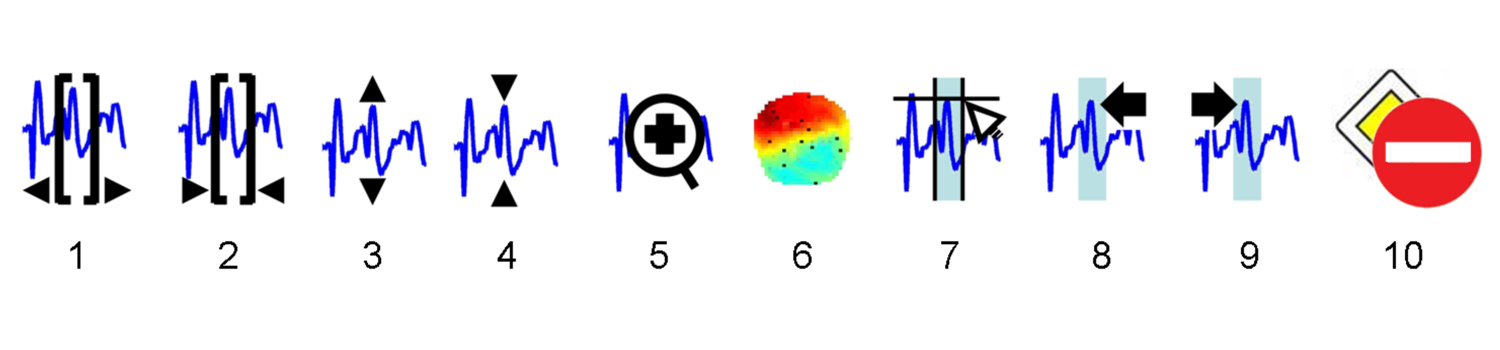
\includegraphics[width=100mm]{meeg/eeg_review_buttons}
\end{center}
\caption{\em SPM M/EEG \textsc{Review} buttons legend 1-2: increase/decrease width of plotted time window, 3-4: increase/decrease global scaling display factor, 5: zoom in, 7: add event, 8-9: scroll backward/forward data from marker to marker, 10: declare event as good/bad}
\end{figure}

\section{Batching and scripts}
Although all functions can be called by the GUI, using only the GUI for preprocessing multi-subject data is a cumbersome and error-prone affair. For this reason, we included functions in SPM8 which should make batching jobs feasible, with only a small amount of \matlab\ knowledge required. How would one batch a series of preprocessing steps in SPM8? There are two ways of doing this, the new batch system of SPM8, and generating scripts.

\subsection{The new SPM8 batch system}
This method uses the new SPM8 batch system described in chapter \ref{Chap:batch_interface}. Using this batch system, you can put together a series of processing steps by choosing options from menus, in any order you like. When the full ``job'' is specified which may be a sequence of several processing step, one executes the job.


\subsection{Script generation}
Another way of batching jobs is by using scripts, written in \matlab\ . In SPM8, you can generate these scripts automatically. To do this, you first have to analyze one data set using the GUI or batch system. In SPM8, whenever a preprocessing function is called, all the input arguments, once they have been assembled by the GUI, are stored in a ``history''. This history can then be used to not only see in detail which functions have been used on a data set, but also to generate a script that repeats the same analysis steps. The big difference is that, this time, no more GUI interactions are necessary because the script already has all the input arguments which you gave during the first run. The history of an \texttt{meeg} object can be accessed by \texttt{D.history}. 
\\
\\
To generate a script from the history of an SPM8 MEEG file, open the file in the M/EEG \textsc{Review} facility and select the \texttt{info} tab: a \texttt{history} tab is then available that will display all the history of the file. Clicking the \textsc{Save as script} button will ask for the filename of the \matlab\ script to save and the list of processing steps to save (default is all but it is possible to select only a subset of them). This will generate a script, which, when run, repeats the analysis. The script can also be obtained by directly calling the function \texttt{spm\_eeg\_history}.
\\
\\
Of course, this script can not only be used to repeat an analysis, but the script can also be seen as a template that can be re-used for other analyses. One needs minimal \matlab\ knowledge for these changes. For example, you can replace the filenames to preprocess a different subject. Or you can change parameters and then re-run the analysis. We have prepared an example, using the same example data set, as in the previous subsection to demonstrate this (see the file \texttt{man$\backslash$example\_scripts$\backslash$history\_subject1.m}). Note that these scripts can currently be used to do things that one couldn't do with the batch system. For example, if you want to exclude a channel from the analysis, there is no way to do this via the batch system. In the GUI, you would have to call display and switch the channel to 'bad'. With a script, you simply add a line like \texttt{D=badchannels(D, 23, 1)}, which flags channel 23 as bad (see also our example script after the filtering step). In summary, the idea is to preprocess a file through the GUI or batch system, then use the history-function to generate a template, and finally adapt this template to modify the analysis in some way. To run the example script on your computer, you need the data set that you can download from the SPM webpage (\footnote{\url{http://www.fil.ion.ucl.ac.uk/spm/data/eeg\_mmn/}}).
